% TEMPLATE.TEX
%
% Time-stamp: <2013-03-26 11:09 olenz>
%
% This is an extensively documented LaTeX file that shows how to
% produce a good-looking document with current LaTeX (11/2012).
%
% IMPORTANT!
%
%   Some obsolete commands and packages
% ----------|-------------------------------
% obsolete  |     Replacement in LATEX 2ε
% ----------|-------------------------------
%           | local            global/switch
% ----------|-------------------------------
% {\bf ...} | \textbf{...}     \bfseries
%     -     | \emph{...}       \em
% {\it ...} | \textit{...}     \itshape
%     -     | \textmd{...}     \mdseries
% {\rm ...} | \textrm{...}     \rmfamily
% {\sc ...} | \textsc{...}     \scshape
% {\sf ...} | \textsf{...}     \sffamily
% {\sl ...} | \textsl{...}     \slshape
% {\tt ...} | \texttt{...}     \ttfamily
%     -     | \textup{...}     \upshape
%
% DON'T USE \\ TO MAKE LINEBREAKS, INSTEAD JUST LEAVE A BLANK LINE!
%
\RequirePackage[l2tabu,orthodox]{nag} % turn on warnings because of bad style
\documentclass[a4paper,10pt,bibtotoc]{scrartcl}
%
\usepackage[bottom=3.5cm, top=2cm]{geometry}
%%%%%%%%%%%%%%%%%%%%%%%%%%%%%%%%%%%%
% KOMA CLASSES
%%%%%%%%%%%%%%%%%%%%%%%%%%%%%%%%%%%%
%
% The class "scrartcl" is one of the so-called KOMA-classes, a set of
% very well done LaTeX-classes that produce a very European layout
% (e.g. titles with a sans-serif font).
%
% The KOMA classes have extensive documentation that you can access
% via the commands:
%   texdoc scrguide # in German
%   texdoc scrguien # in English
%
%
% The available classes are:
%
% scrartcl - for "articles", typically for up to ~20 pages, the
%            highest level sectioning command is \section
%
% scrreprt - for "reports", typically for up to ~200 pages, the
%            highest level sectioning command is \chapter
%
% scrbook  - for "books", for more than 200 pages, the highest level
%            sectioning command is \part.
%
% USEFUL OPTIONS
%
% a4paper  - Use a4 paper instead of the default american letter
%            format.
%
% 11pt, 12pt, 10pt
%          - Use a font with the given size.
%
% bibtotoc - Add the bibliography to the table of contents
%
% The KOMA-script classes have plenty of options to modify

% This allows to type UTF-8 characters like ä,ö,ü,ß
\usepackage[utf8]{inputenc}

\usepackage[T1]{fontenc}        % Tries to use Postscript Type 1 Fonts for better rendering
\usepackage{lmodern}            % Provides the Latin Modern Font which offers more glyphs than the default Computer Modern
\usepackage[intlimits]{amsmath} % Provides all mathematical commands

\usepackage{hyperref}           % Provides clickable links in the PDF-document for \ref
\usepackage{graphicx}            % Allow you to include images (like graphicx). Usage: \includegraphics{path/to/file}

% Allows to set units
\usepackage[ugly]{units}        % Allows you to type units with correct spacing and font style. Usage: $\unit[100]{m}$ or $\unitfrac[100]{m}{s}$

% Additional packages
\usepackage{url}                % Lets you typeset urls. Usage: \url{http://...}
\usepackage{breakurl}           % Enables linebreaks for urls
\usepackage{xspace}             % Use \xpsace in macros to automatically insert space based on context. Usage: \newcommand{\es}{ESPResSo\xspace}
\usepackage{xcolor}             % Obviously colors. Usage: \color{red} Red text
\usepackage{booktabs}           % Nice rules for tables. Usage \begin{tabular}\toprule ... \midrule ... \bottomrule

% Source code listings
\usepackage{listings}           % Source Code Listings. Usage: \begin{lstlisting}...\end{lstlisting}
\lstloadlanguages{python}
\definecolor{lightpurple}{rgb}{0.8,0.8,1}

\lstset{
stepnumber=1,
numbersep=5pt,
numberstyle=\small\color{black},
basicstyle=\ttfamily,
%keywordstyle=\color{black},
%commentstyle=\color{black},
%stringstyle=\color{black},
frame=single,
tabsize=4,
language = python,
backgroundcolor=\color{black!5}}

\usepackage{float}

\begin{document}

\titlehead{Simulation Methods in Physics II \hfill SS 2020}
\title{Report for Worksheet 2: Properties of water from quantum mechanical and atomistic simulation}
\author{Markus Baur and David Beyer}
\date{\today}
\maketitle

\tableofcontents

\section{Short Questions --Short Answers}
\begin{itemize}
\item \textbf{A1}: Water molecules consist of one oxygen atom (O) and two hydrogen atoms (H). Because oxygen has a much higher electronegativity (i.e a tendency to attract bond electrons towards itself) than hydrogen, water molecules exhibit positive partial charges at the hydrogen atoms and negative partial charges at the oxygen atoms. A dipole moment arises (i.e the molecules are polar) because of the non-linear (bent) molecular structure.

\item \textbf{A2}: A hydrogen bond is a weak bond (compared to covalent or ionic bonds) which arises between a (partially positively charged) hydrogen atom (as part of a molecule) and partially negatively charged atom like oxygen (e.g. in water, i.e also part of a molecule). Hydrogen bonds can be intermolecular (e.g. in water) or intramolecular (e.g. in DNA or proteins).

\item \textbf{A3}: The H--O--H angle in water molecules is about 104.45$^\circ$.\footnote{https://en.wikipedia.org/wiki/Properties\_of\_water, accessed on May 8 2020, 20:00} Hydrogen bonds in water have a typical length of 1.97$\r{A}$.\footnote{http://chemistry.elmhurst.edu/vchembook/161Ahydrogenbond.html, accessed on May 8 2020, 20:00}

\item \textbf{A4}: SPC, SPC/E and TIP3P are all 3-site water models, meaning that they include partial charges at three sites in the molecule. SPC and SPC/E have a bond length of 1.0$\,$\r{A} and an angle of 109.47$^\circ$ (tetrahedral) while TIP33P has a bond length of 0.9572$\,$\r{A} and an angle of 104.52$^\circ$. The partial charges and strength of the Lennard-Jones interaction also vary between the models. The difference between SPC and SPC/E is that SPC/E also includes an average polarization energy.
\end{itemize}

\section{Quantum Mechanical Calculation of Water}
\subsection{Quantum Mechanical Calculation of Water}
We performed simulations of the water dimer using the PBE functional and the LDA functional, both with and without a van der Waals interaction. 
A visualization of the water dimer is shown in \autoref{fig:fig_dimer}.
The obtained bond lengths are shown in \autoref{tab0}.
To calculate these bond lengths, we used the output data in the position file and wrote the python script bond\_lengths.py. 
The OH-bond lengths which are shown in the table were averaged over all four bonds.
The van der Waals interaction seems to have no influence on the length of the covalent O-H bond, while it seems to vary with the used functional. Both PBE and LDA overestimate the length of the covalent O-H bond (the experimental value is about $0.95\,\r{A}$). 
For the hydrogen bond, the used exchange correlation functional also seems to be much more important than the van der Waals interaction. 
LDA heavily underestimates the length of the hydrogen bond (experimental value $1.97\,\r{A}$) while PBE is quite close to the experimental value.

\begin{figure}[h]
\centering
 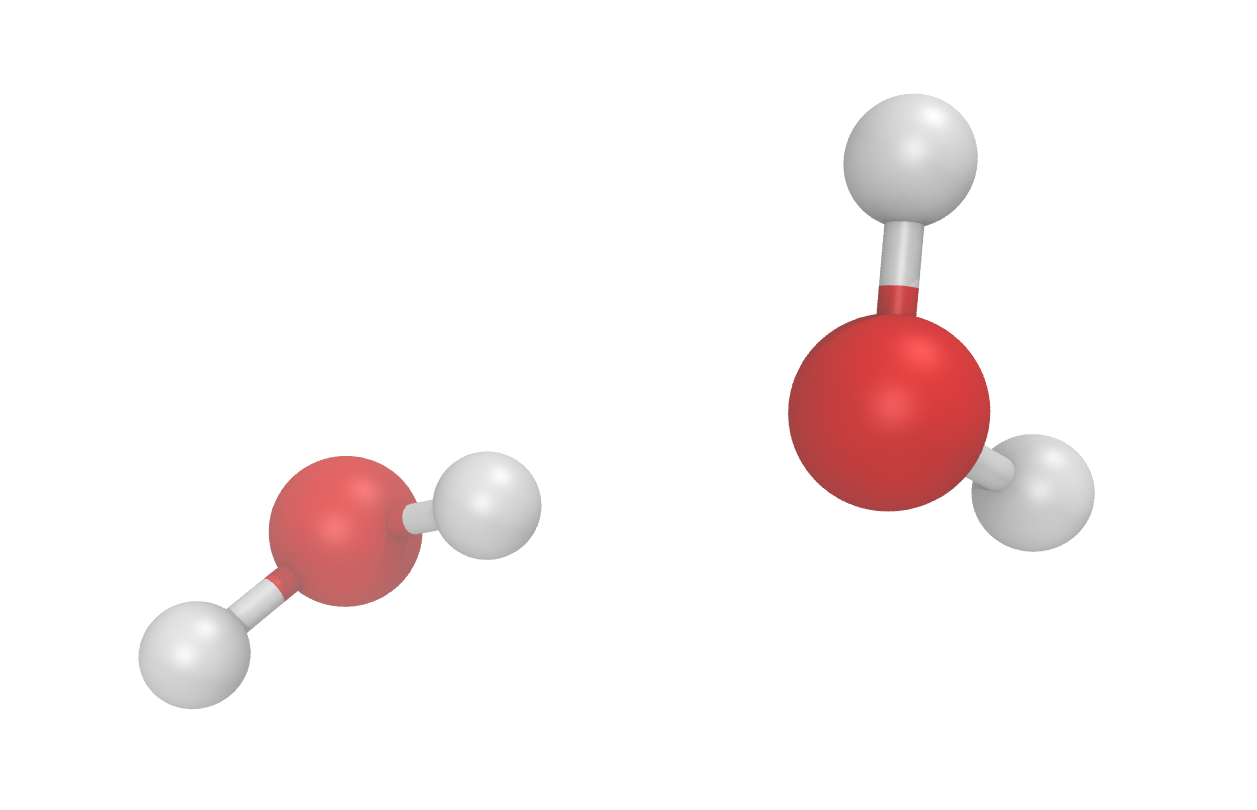
\includegraphics[width=0.6\textwidth]{dimer.png}
 \caption{Visualization of the water dimer, it has a hydrogen bond.}
 \label{fig:fig_dimer}
\end{figure}

\begin{table}[h]
\centering
\caption{Bond lengths for different functionals.}
\begin{tabular}{@{}lcc@{}}
\toprule
functional & length of O-H bond $\left[\r{A}\right]$ & length of hydrogen bond $\left[\r{A}\right]$ \\ \midrule
PBE with vdW       & 0.9745 & 1.9379                 \\
PBE without vdW       & 0.9745
 & 1.9380    \\
LDA with vdW       & 0.9777 & 1.7470              \\ 
LDA without vdW & 0.9777& 1.7429\\\bottomrule
\end{tabular}
\label{tab0}
\end{table}


\noindent We performed simulations of the water monomer using the PBE functional and the LDA functional, both with and without a van der Waals interaction. 
The obtained Hirshfeld charges of O and H are shown in \autoref{tab}.
Again, there is a difference between the two different functionals.

\begin{table}[h]
\centering
\caption{Hirshfeld charges of O and H for different functionals.}
\begin{tabular}{@{}lcc@{}}
\toprule
functional & Hirshfeld charge of O $\left[e\right]$ & Hirshfeld charge of H $\left[e\right]$ \\ \midrule
PBE with vdW       & -1.108 & 0.560                 \\
PBE without vdW       & -1.108 & 0.560            \\
LDA with vdW       & -1.127 & 0.570              \\ 
LDA without vdW & -1.127 & 0.570\\\bottomrule
\end{tabular}
\label{tab}
\end{table}

\subsection{Ab Initio Molecular Dynamics Simulation of Water Dimer}
We performed ab initio molecular dynamics simulations of the water monomer and dimer using the PBE functional at temperatures $T\in\{100\,\mathrm{K}, 200\,\mathrm{K}, 300\,\mathrm{K}\}$. 
The time step was set to $0.5\,\mathrm{fs}$. 
We the ran the simulations for $T=100\,\mathrm{K}$ and $T=200\,\mathrm{K}$ for about 3000 steps.
The simulations for $T=300\,\mathrm{K}$ were run for about 10000 steps.

To calculate the mean potential energy of the hydrogen bond of the water dimer, we have to subtract the mean energy of two water monomers from the mean energy of the water dimer:
\begin{align}
\langle E_\mathrm{pot,H-bond}\rangle = \langle E_\mathrm{pot,dimer}\rangle - 2\cdot \langle E_\mathrm{pot,monomer}\rangle .
\end{align}
In order to calculate the mean potential energy for a given trajectory, we wrote the python script energies.py. 
The calculated mean potential energies for the hydrogen bonds are shown in \autoref{tab_hbond_energy}.
As we would expect, the mean potential energy of the hydrogen bond decreases for higher temperatures because of thermal fluctuations.

\begin{table}[h]
\centering
\caption{Mean potential energy of the hydrogen bond $\langle E_\mathrm{pot,H-bond}\rangle$ in eV.}
\begin{tabular}{@{}cc@{}}
\toprule
temperature $T$ $\left[\mathrm{K}\right]$ & $\langle E_\mathrm{pot,H-bond}\rangle$ $\left[\mathrm{eV}\right]$\\ \midrule
100         &   -0.21609\\
200        &  -0.19848\\
300      &     -0.15977\\ \bottomrule
\end{tabular}
\label{tab_hbond_energy}
\end{table}

\noindent In order to calculate the mean length of the hydrogen bond, we wrote the python script\\ mean\_bond\_lengths.py.
The calculated mean lengths of the hydrogen bonds are shown in \autoref{tab_hbond_length}.
As expected, the bond length increases with temperature (the input structure corresponds to zero temperature).

\begin{table}[h]
\centering
\caption{Length of the hydrogen bond for different temperatures.}
\begin{tabular}{@{}cc@{}}
\toprule
temperature $T$ $\left[\mathrm{K}\right]$ &  mean length of hydrogen bond $\left[\r{A}\right]$\\ \midrule
100  &  2.0006\\
200  &  2.8513\\
300  &  3.0573\\
input structure & 1.9758
\\\bottomrule
\end{tabular}
\label{tab_hbond_length}
\end{table}
\subsection{Infrared Spectroscopy}
In order ot calculate the infrared absorption cross-section numerically, we wrote the Python script infrared.py. 
The results are shown in \autoref{fig:fig_monomer_spectrum} and \autoref{fig:fig_dimer_spectrum}.
The spectrum of the water monomer consists of much sharper lines than the spectrum of the dimer, probably because the dimer has more eigenmodes.
\begin{figure}[H]
\centering
\includegraphics[width=\textwidth]{monomer.pdf}
 \caption{Absorption cross-section for the water monomer.}
 \label{fig:fig_monomer_spectrum}
 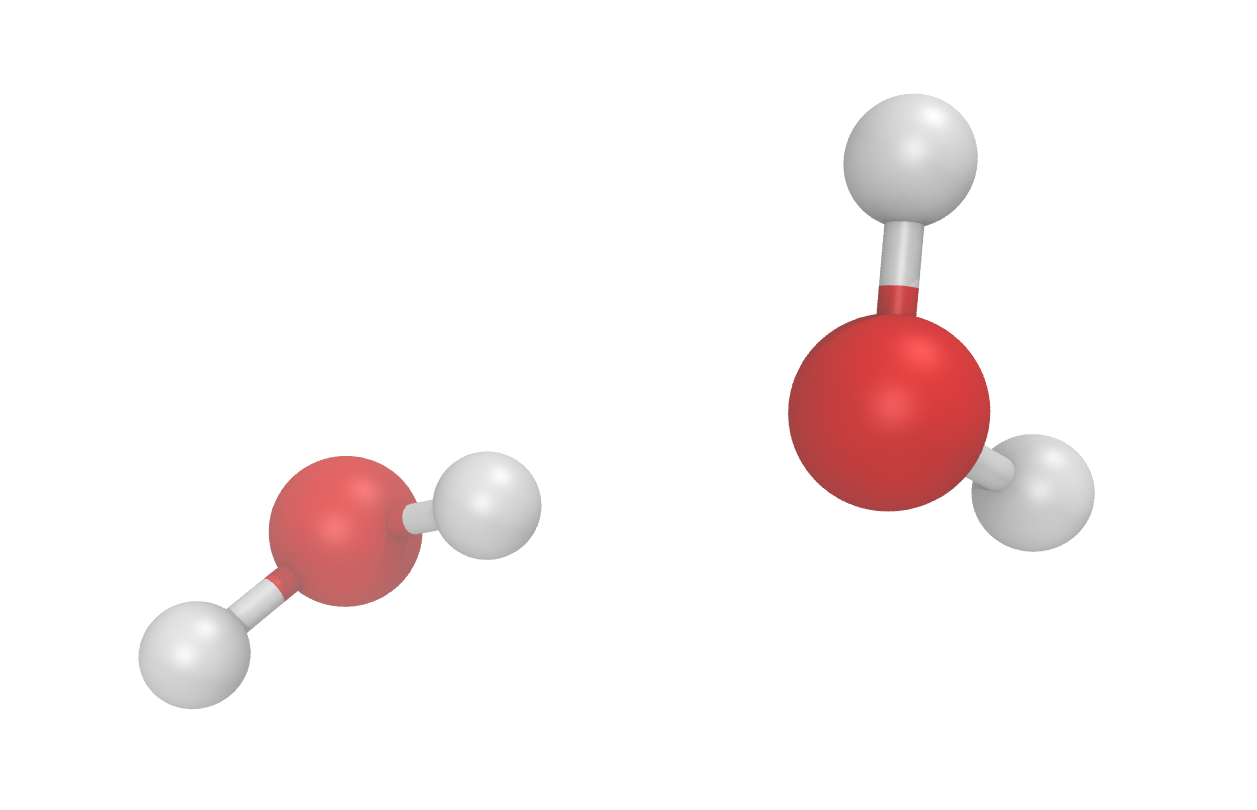
\includegraphics[width=\textwidth]{dimer.pdf}
 \caption{Absorption cross-section for the water dimer.}
 \label{fig:fig_dimer_spectrum}
\end{figure}



\newpage
\section{Atomistic Simulation of Water}
\subsection{Running the Simulations}
We performed atomistic simulations of 216 water molecules using GROMACS and three different water models (SPCE, SPCE/E and TIP3P). The temperature was set to $T=300\,\mathrm{K}$ and the simulations were run for 250000 time steps of size $\Delta t = 2\,\mathrm{fs}$.

\subsection{Analysis}
\subsubsection*{Radial Distribution Function}
\autoref{fig:fig_gromacs_1} -- \autoref{fig:fig_gromacs_3} show the calculated radial distribution functions for the different water models.
On a qualitative level, they all look like we would expect the RDF of a fluid to look like: for small radii, the RDF is zero because two water molecules can never occupy the same place. 
Then comes the highest peak due to the water molecules in the immediate neighbourhood. 
For even larger radii there are (damped) oscillations of the RDF because of particles in even larger ``shells'', the damping is due to the fact that a fluid exhibits no long-range order. 
In the limit $r\rightarrow \infty$, the RDF approaches the value 1.0, because there are no long-range correlations in fluids.
\autoref{fig:fig_rdf} shows how particles arrange around a particle in a fluid, leading to this characteristic behaviour.

While the different RDFs agree on a qualitative level, the peaks for SPC and SPCE are damped much weaker than for TIP3P, this suggest that the fluid phase for the former two is somehow more ordered than for TIP3P.

\begin{figure}[h]
\centering
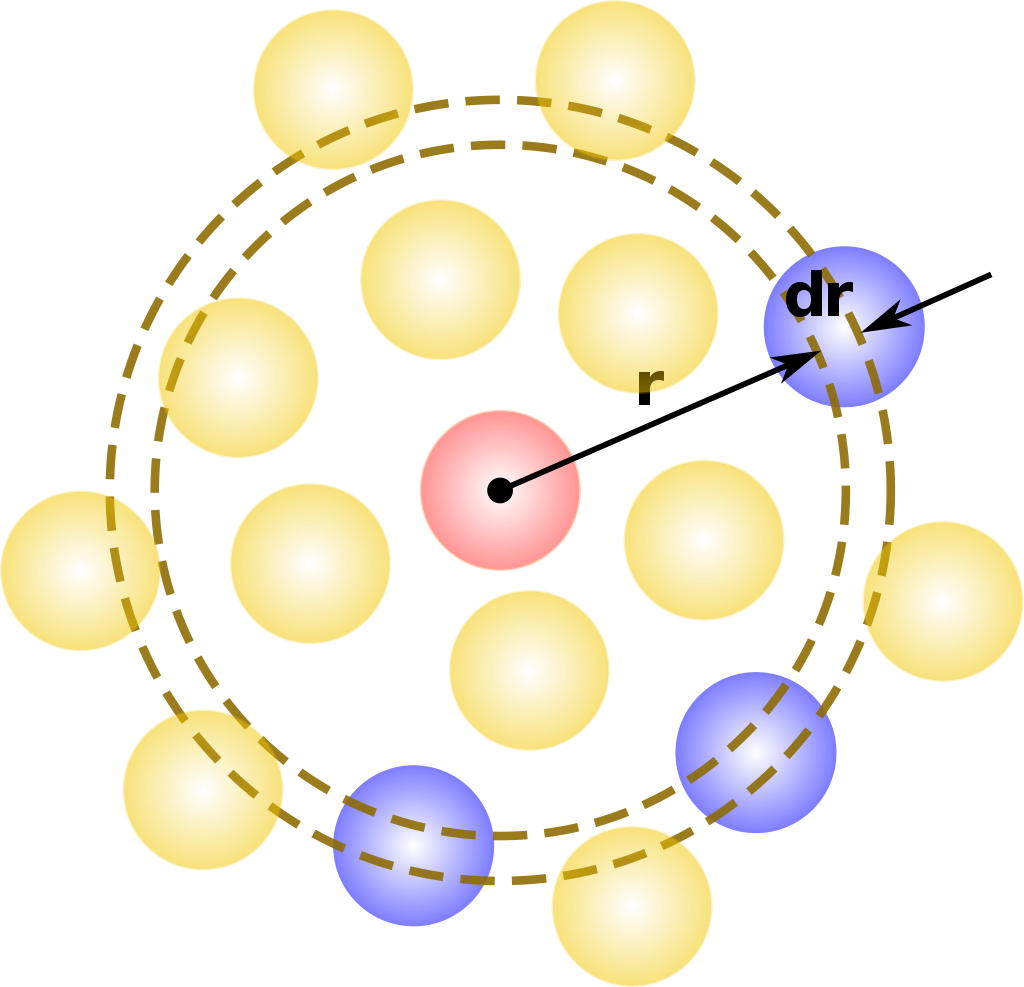
\includegraphics[width=0.5\textwidth]{1024px-Rdf_schematic.png}
\caption{Schematic explanation of the RDF. (Taken from \texttt{https://commons.wikimedia.org/wiki/File:Rdf\_schematic.svg}, accessed on May 18, 2020 at 8:00 pm.)}
\label{fig:fig_rdf}
\end{figure}

\begin{figure}[h]
\centering
 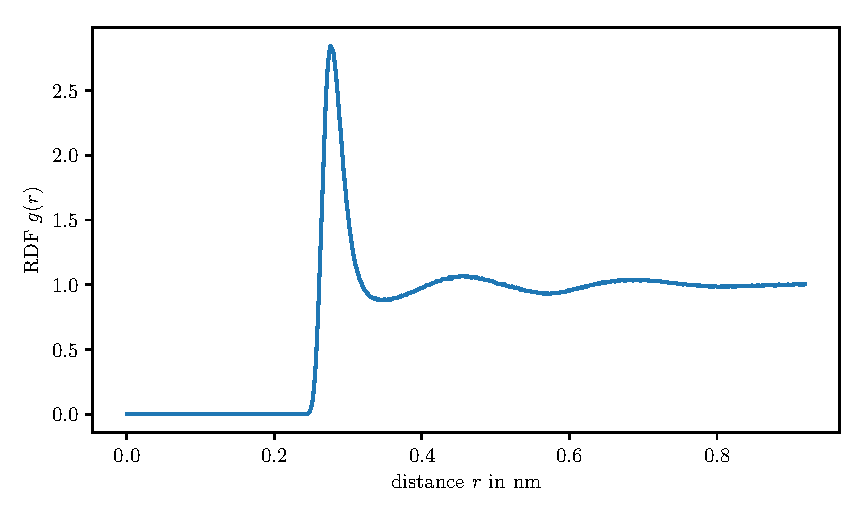
\includegraphics[width=0.8\textwidth]{RDF_SPC.pdf}
 \caption{Radial distribution function for the SPC water model.}
 \label{fig:fig_gromacs_1}
 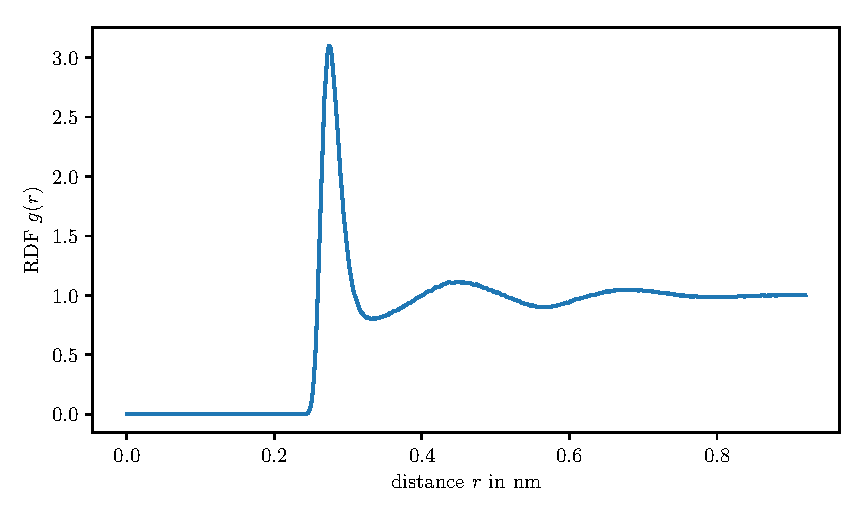
\includegraphics[width=0.8\textwidth]{RDF_SPCE.pdf}
 \caption{Radial distribution function for the SPCE water model.}
 \label{fig:fig_gromacs_2}
 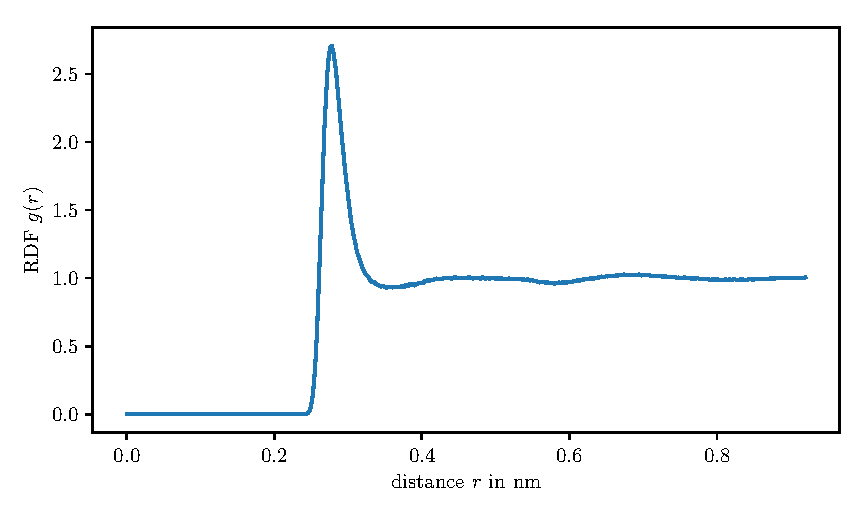
\includegraphics[width=0.8\textwidth]{RDF_TIP3P.pdf}
 \caption{Radial distribution function for the TIP3P water model.}
 \label{fig:fig_gromacs_3}
\end{figure}

\subsubsection*{Hydrogen Bond Analysis}
The number of hydrogen bonds per water molecule for the three different water models is shown in \autoref{tab1}.

\begin{table}[h]
\centering
\caption{Average number of hydrogen bonds per water molecule for different water models.}
\begin{tabular}{@{}cc@{}}
\toprule
water model & avg. number of H-bonds \\ \midrule
SPC         &          1.73                 \\
SPCE        &          1.80               \\
TIP3P       &          1.67                 \\ \bottomrule
\end{tabular}
\label{tab1}
\end{table}

\subsubsection*{Mean Square Displacement and Diffusion Coefficient}
\autoref{fig:fig_gromacs_4}--\autoref{fig:fig_gromacs_6} show plots of the mean square displacement which was computed for the different water models. 
For larger values of $t$, the MSD begins to oscillate stronger and stronger due to the fact that there are less samples available. 
We can clearly see that the slope (i.e. the diffusion coefficient) for TIP3P is by far the largest while for SPC/E it is the smallest.

\noindent To identify the ballistic regime, we plot the MSD on log-log plot (\autoref{fig:fig_gromacs_7}--\autoref{fig:fig_gromacs_9}). 
For all three models there is a change in the slope which points to change in the power law $t^n$. 
To investigate the behaviour for $t\rightarrow 0$, we fitted a power law $a\cdot t^n$ to the first few data points of each model.
The obtained fits are also shown in the respective figures.
\autoref{tab3} shows the exponents which were extracted from the fits.
While they are all larger than 1, they are still smaller than the value we would expect for purely ballistic motion ($n=2$).

\begin{table}[h]
\centering
\caption{Computed power law exponents in the short time limit for the different water models}
\begin{tabular}{@{}cc@{}}
\toprule
water model & power law exponent $n$ \\ \midrule
SPC         & 1.240\\
SPCE        & 1.253\\
TIP3P       & 1.255\\ \bottomrule
\end{tabular}
\label{tab3}
\end{table}

\noindent GROMACS uses a fitting range of $\left[50\,\mathrm{ps},450\,\mathrm{ps}\right]$ which seems sensible given the fact that there is a non-diffusive regime for small $t$ and larger fluctutations for large $t$. 
The computed diffusion coefficients are given in \autoref{tab2}, while they are not exactly equal, they are of the same order of magnitude. 

\begin{table}[h]
\centering
\caption{Computed diffusion coefficients for the different water models}
\begin{tabular}{@{}cc@{}}
\toprule
water model & diffusion coefficient $D$ in $10^{-5}\,\mathrm{cm}^2\cdot \mathrm{s}^{-1}$ \\ \midrule
SPC         &          3.7948 $\pm$ 0.1089                 \\
SPCE        &          2.2704 $\pm$ 0.1190            \\
TIP3P       &          5.0608 $\pm$       0.3821    \\ \bottomrule
\end{tabular}
\label{tab2}
\end{table}


\begin{figure}[h]
\centering
 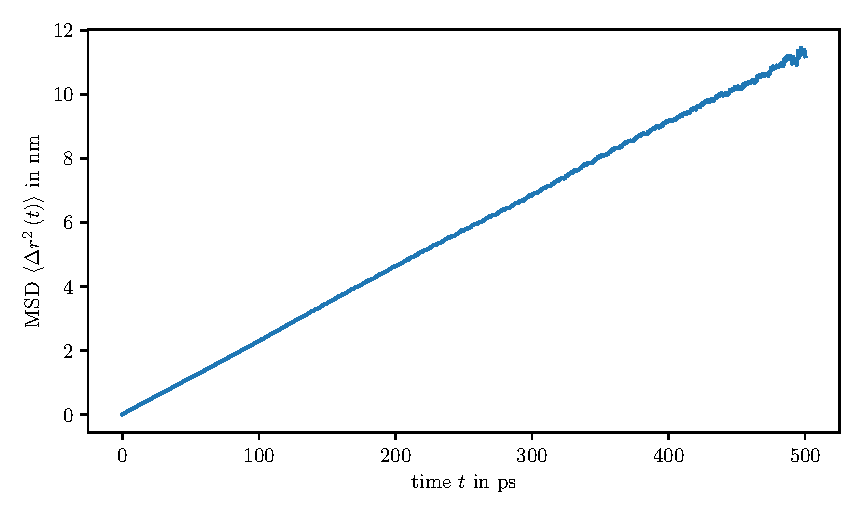
\includegraphics[width=0.8\textwidth]{MSD_SPC.pdf}
 \caption{Mean square displacement for the SPC water model.}
 \label{fig:fig_gromacs_4}
 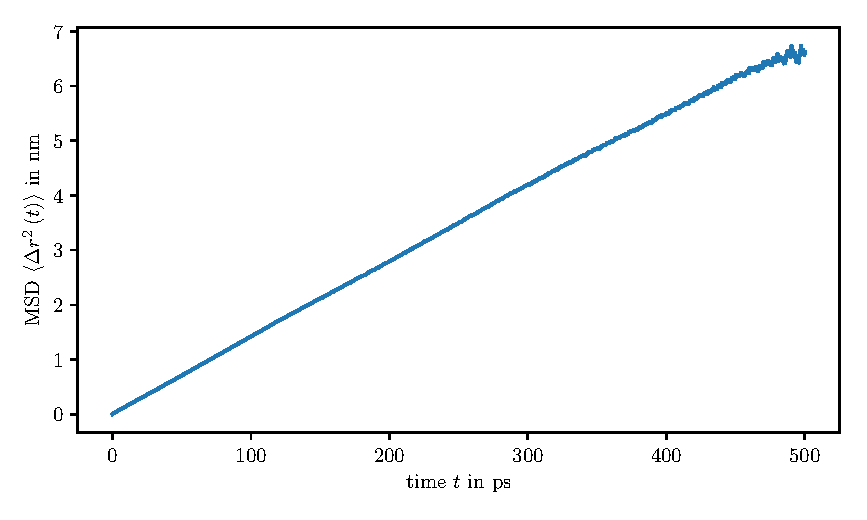
\includegraphics[width=0.8\textwidth]{MSD_SPCE.pdf}
 \caption{Mean square displacement for the SPCE water model.}
 \label{fig:fig_gromacs_5}
 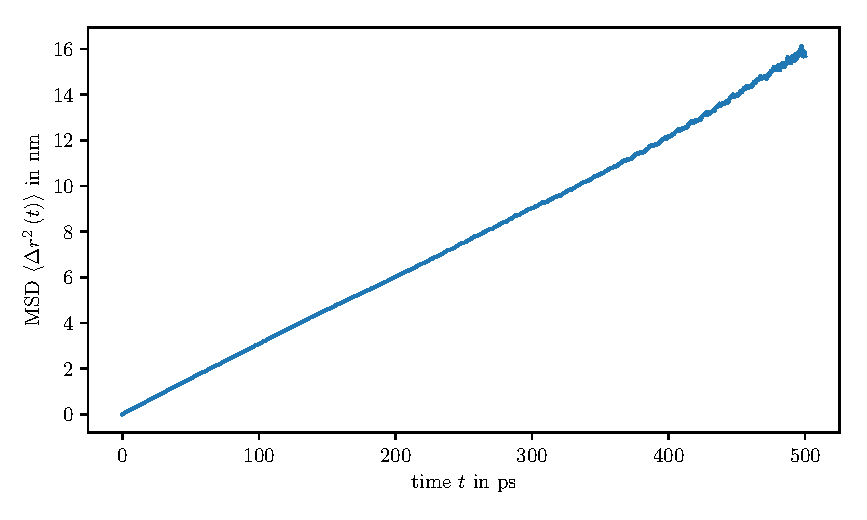
\includegraphics[width=0.8\textwidth]{MSD_TIP3P.pdf}
 \caption{Mean square displacement for the TIP3P water model.}
 \label{fig:fig_gromacs_6}
\end{figure}

\begin{figure}[h]
\centering
 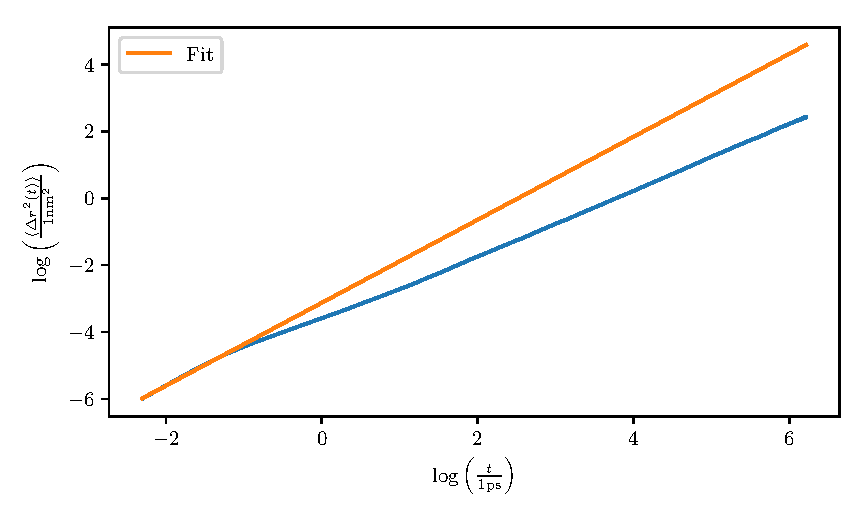
\includegraphics[width=0.8\textwidth]{MSD_SPC_LOG.pdf}
 \caption{Log-log plot of the mean square displacement for the SPC water model.}
 \label{fig:fig_gromacs_7}
 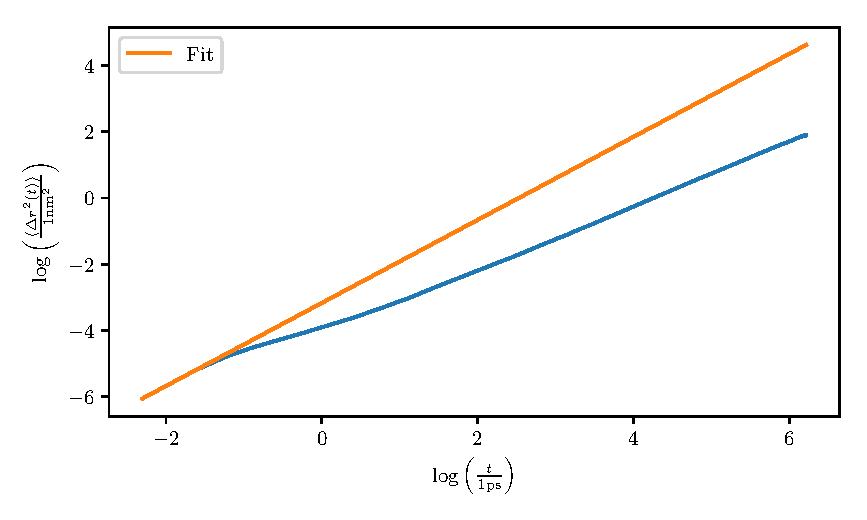
\includegraphics[width=0.8\textwidth]{MSD_SPCE_LOG.pdf}
 \caption{Log-log plot of the mean square displacement for the SPCE water model.}
 \label{fig:fig_gromacs_8}
 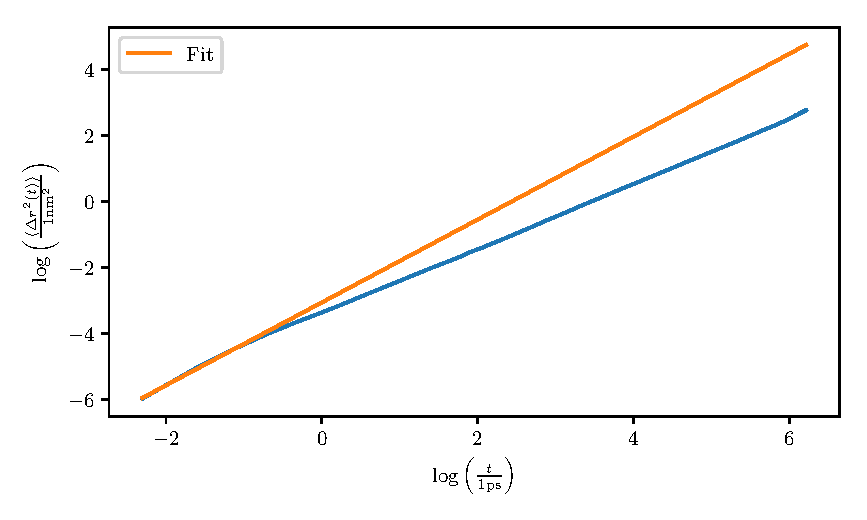
\includegraphics[width=0.8\textwidth]{MSD_TIP3P_LOG.pdf}
 \caption{Log-log plot of the mean square displacement for the TIP3P water model.}
 \label{fig:fig_gromacs_9}
\end{figure}

\end{document}
